\documentclass{article}

\usepackage[L7x,T1]{fontenc}
\usepackage[utf8]{inputenc}
\usepackage[lithuanian]{babel}
\usepackage{hyperref}
\usepackage{minted}
\usepackage{tikz}
\usetikzlibrary{positioning}

\title{Žemėlapių naršyklės ir elektroninės paslaugos\\ \vspace{4mm} 
Galutinis semestro egzaminas}

\author{Motiejus Jakštys}

\date{\today}

\begin{document}
\maketitle

\section{Įžanga}

Kaip pasufleruota užduotyje, pagrindinė problema yra bandymas atvaizduoti per
daug duomenų vienu metu. Problemos sprendimas dvilypis: vartotojo sąsajoje ir
"serverinėje" implementacijoje.

Kaip pasufleruota užduotyje, sprendimas dvilypis: vartotojo sąsaja ir serverinis komponentas.

\section{Sprendimas}

Kadangi problema labai opi smulkiuose masteliuose, pirmiausia nuspręskime, kaip
žemėlapį vaizduoti smulkiame mastelyje. Tai atsispindės ir GUI/UX, ir
serveriniame sprendime.

\subsection{Funkcionalumo keitimas, GUI/UX keitimas}
\label{sec:ux}

Jei vienoje vietoje (pvz., per 5\% ekrano ploto) yra daugiau, nei du objektai,
juos agreguoti ir vietoj pačių objektų rodyti skaičių, kiek tame plote yra
objektų. Tada priartinus tuos objektus jie natūraliai atsiskirs.

Tai implementuojant reikia apgalvoti šiokias tokias išimtis: pvz., jei ekrane
rodoma iš viso mažiau, nei X objektų (tarkime, 42), tuomet agregacijos daryti
nereikia, ir rodyti viską taip, kaip buvo "senuoju būdu". Taip užtikriname, kad
objektus, kad ir kaip arti vienas kito esančius, visada galėsime pamatyti
pakankamai priartinę. Algoritmą, kaip tai padaryti, aprašome
skyriuje~\ref{sec:backend}.

\subsection{Žemėlapio vizualizacijos modifikavimo/optimizavimo priemonės}
\label{sec:api}

Šioje sekcijoje aprašome API dalį: į ką pakeisti milžinišką GeoJSON objektą,
kad galėtume jį atvaizduoti?

Pirmiausia, vartotojas į serverį turi siųsti savo matomo žemėlapio koordinates
({\em extent}). Tada pagal tai serveris nusprendžia, kuriuos duomenis grąžinti
tiesiogiai, kuriuos -- agreguotus. Taip kai kurie taškai lieka originalūs, o
kai kurie dingsta, ir vietoje jų atsiranda "agreguoti".

Agreguoti taškai -- GeoJSON objektai, tačiau su papildomu atributu, kad tai yra
"virtualūs" taškai, ir nurodantys, kiek objektų savyje "slepia". Pvz.

\begin{minted}{json}
{
  "type": "Feature",
  "geometry": {
    "type": "Point",
    "coordinates": [24.3 55.68]
  },
  "properties": {
    "aggregated": true,
    "aggregate_count": 10
  }
}
\end{minted}

Paspaudus ant agreguoto komponento būtų patogu, jei atsirastų kitas langas su
visais "slepiamais" komponentais, arba žemėlapis taip prisiartintų, kad
pasirodytų visi to agreguoto vidiniai slepiami objektai.

Grąžinus tik matomą dalį duomenų, serveris visada atsiųs pakankamai mažą kiekį
GeoJSON objektų, kurie tikrai neapkraus naršyklės; taip vartotojo sąsaja bus
sėkmingai naudotina ir smulkiuose, ir stambiuose masteliuose.

\subsection{Esamų servisų modifikavimo ir/ar naujų kūrimo priemonės, įvardinant
konkrečius servisus tipus/sprendimus ir juos trumpai pagrindžiant}

Dėstytojo nurodymu, ArcGIS Online pakeičiame PostGIS duombaze ir serveriniu
({\em back-end}) komponentu; žr. architektūros diagramą~\ref{fig:arch}.

\begin{figure}[H]
    \centering
    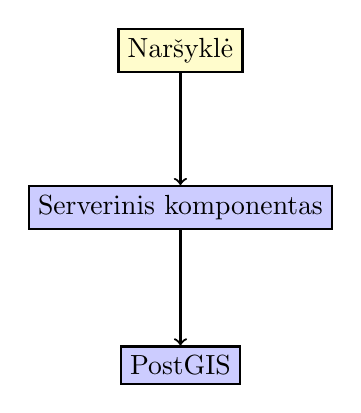
\begin{tikzpicture}[thick]
        \node at (0,4)[rectangle,draw=black,fill=yellow!20] (browser) {Naršyklė};
        \node at (0,2)[rectangle,draw=black,fill=blue!20] (backend) {Serverinis komponentas};
        \node at (0,0)[rectangle,draw=black,fill=blue!20] (gis) {PostGIS};
        \draw [->] (browser) to (backend);
        \draw [->] (backend) to (gis);
    \end{tikzpicture}
    \caption{Architektūros diagrama}
    \label{fig:arch}
\end{figure}

Pakeitę ArcGIS į PostGIS, atsikratome dirbtinio 2000 objektų ribojimo ir
aplikacijoje galime pasiimti tiek duomenų, kiek reikia. Šioje užduotyje taip
pat tariame, kad visi, kas įrašinėja objektus, juos rašo į duombazę naudojant
GIS įrangą, ir įrašymu mums rūpintis nereikia.

Liko neišspręsta viena problema: kaip, turint tūkstančius objektų ir vartotojo
"langą" (extent) grąžinti tinkamus PostGIS objektus? Logiką galima dėti į dvi
vietas: arba duomenų bazę, arba pačią programą.

\subsubsection{Duomenų bazė}
\label{sec:db}

Programuoti skirstymo duomenų bazėje yra paprasčiau, nei serveriniame
komponente. Pavyzdinis, gana naivus, algoritmas, kurį galima parašyti naudojant
plpgsql:

\begin{itemize}
    \item parinkti objektus, esančius rėme ({\em extent}).
    \item padalinti rėmą į reikiamą skaičių dalių (aprašyta~\ref{sec:ux}). Rėmą
        populiaru dalinti į šešiakampius arba kvadratus.

    \item kiekvienai daliai grąžinti tikrus arba virtualius objektus
        (aprašyta~\ref{sec:api}).

    \item sukonstruoti GeoJSON objektą ir grąžinti vartotojui.
\end{itemize}

Nors išspręsti problemą duomenų bazėje yra paprasčiau kodo prasme, tačiau
duomenų bazės apkrovimas bus didesnis ir kils su naršančiųjų kiekiu. Todėl
ateityje, jei duomenų arba vartotojų bus dar daugiau, gali būti sunkiau
optimizuoti algoritmus; naudojant tikrą programavimo kalbą (tarkime, C++ arba
Go) daug paprasčiau optimizuoti ir užtikrinti norimą servisą augant vartotojų
skaičiui.

\subsubsection{Serverinis komponentas}
\label{sec:backend}

Algoritmas gali būti panašus į aprašytą~\ref{sec:db}. Tačiau kaip gauti
duomenis?

Kadangi objektų kiekis -- tik dešimtys tūkstančių, visus duomenis lengvai
galima laikyti atmintyje ir serveriniame komponente analizę leisti su kiekviena
užklausa iš naujo. Duomenis atsisiųsti iš duomenų bazės galima reguliariai,
tarkime, kas kelias sekundes ar minutę: taip duomenų bazės apkrovimas bus
minimalus, ir nekils didėjant skaitytojų kiekiui (didės rašančiųjų kiekiui, bet
tokių paprastai būna daug mažiau).

Kaip minėta anksčiau, serveriniame komponente lengviau užtikrinti, kad servisas
veiks gerai ir su dideliais apkrovimais, ir nereikės didinti duomenų bazių
galingumo, kas paprastai yra brangiau ir/arba sudėtingiau, nei aplikacijos.

Jei apkrovimai smarkiai didėja, reikia analizuoti ir tobulinti algoritmą.
Kelios idėjos optimizacijai:

\begin{itemize}

    \item apskaičiuoti generalizacijas iš anksto kiekvienam įmanomam masteliui
        ir atėjus užklausai, tiesiog pasiimti jas iš atminties.

    \item išankstinės optimizacijos, jei skaičiuojamos ne kiekvienos užklausos
        metu, gali būti leidžiamos ir į duomenų bazę: taip DB apkrovimas
        nesikeičia su naršančių vartotojų kiekiu.

\end{itemize}

\end{document}
